\section{CFd\-Reactor  Class Reference}
\label{classCFdReactor}\index{CFdReactor@{CFd\-Reactor}}
{\tt \#include $<$CFd\-Reactor.h$>$}

Inheritance diagram for CFd\-Reactor::\begin{figure}[H]
\begin{center}
\leavevmode
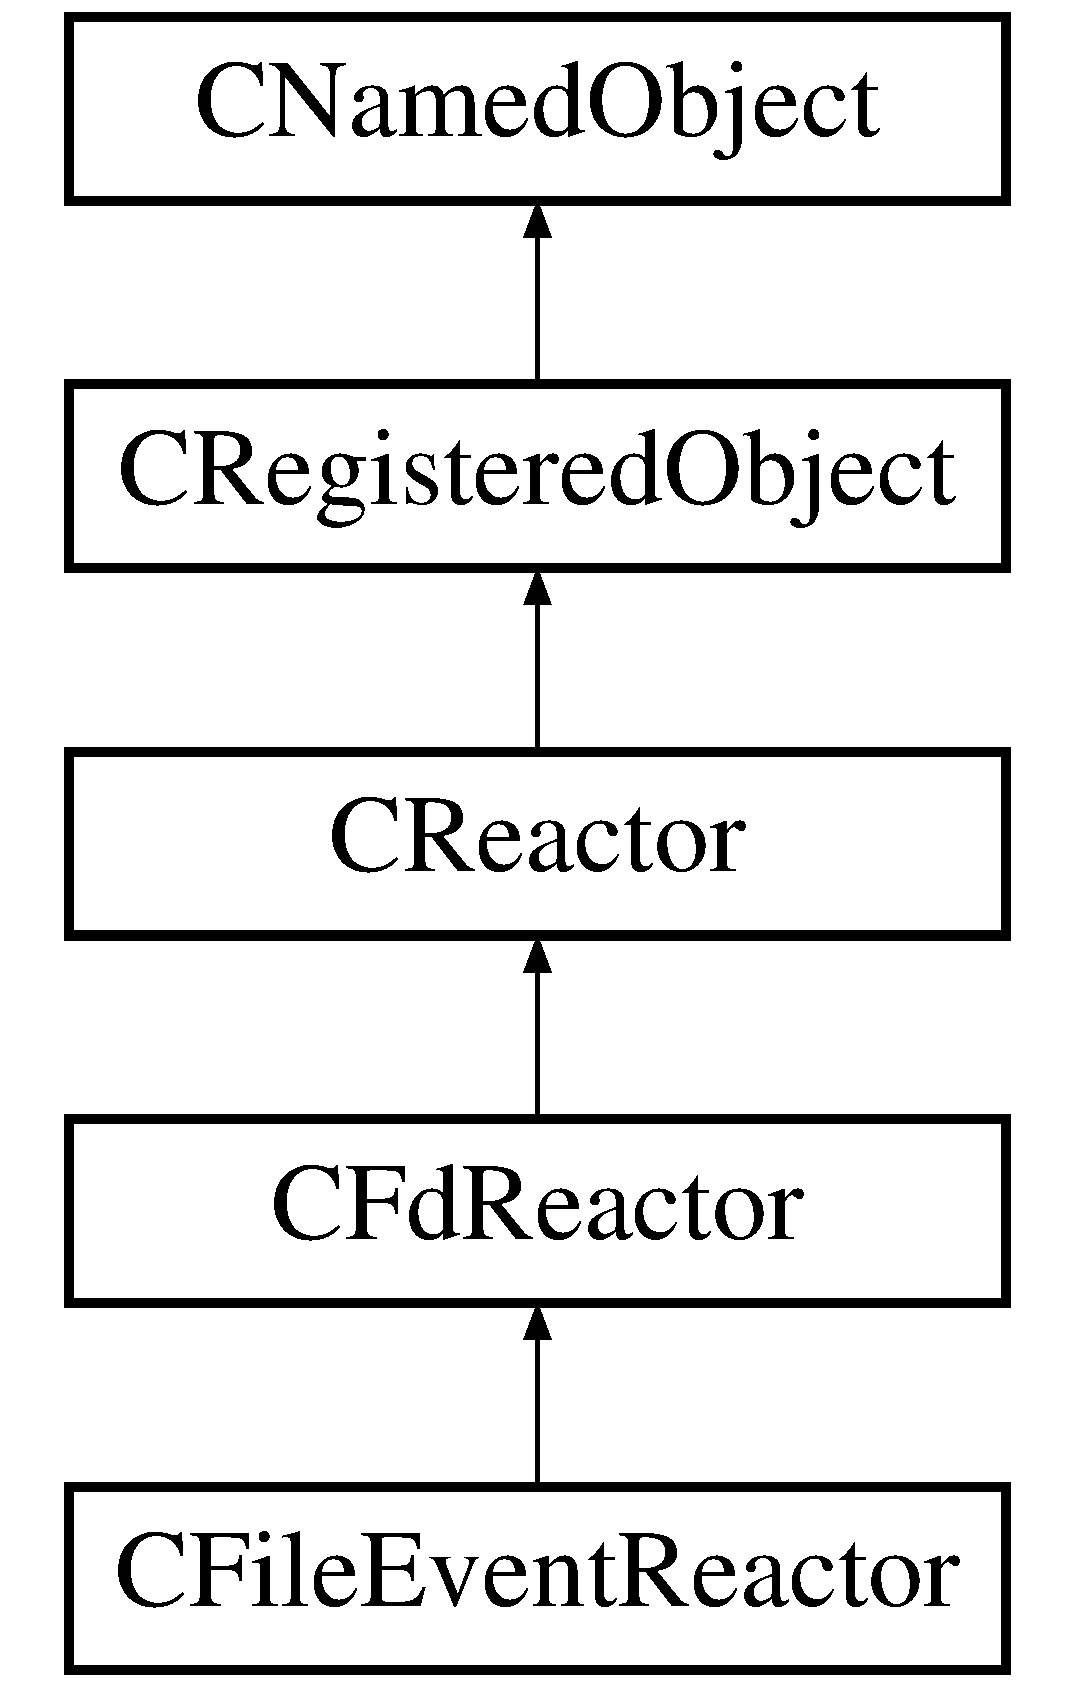
\includegraphics[height=5cm]{classCFdReactor}
\end{center}
\end{figure}
\subsection*{Public Methods}
\begin{CompactItemize}
\item 
{\bf CFd\-Reactor} ()
\item 
{\bf CFd\-Reactor} (const char $\ast$p\-Name)
\item 
{\bf CFd\-Reactor} (const string \&r\-Name)
\item 
virtual {\bf $\sim$CFd\-Reactor} ()
\item 
int {\bf operator==} (const CFd\-Reactor \&a\-CFd\-Reactor) const
\begin{CompactList}\small\item\em Operator== Equality Operator.\item\end{CompactList}\item 
virtual void {\bf On\-Event} ({\bf CEvent\-Monitor} \&r\-Monitor)
\item 
virtual void {\bf On\-Readable} ({\bf CFd\-Monitor} \&r\-Monitor, int fd)
\item 
virtual void {\bf On\-Writable} ({\bf CFd\-Monitor} \&r\-Monitor, int fd)
\item 
virtual void {\bf On\-Exception} ({\bf CFd\-Monitor} \&r\-Monitor, int fd)
\end{CompactItemize}
\subsection*{Private Methods}
\begin{CompactItemize}
\item 
{\bf CFd\-Reactor} (const CFd\-Reactor \&a\-CFd\-Reactor)
\begin{CompactList}\small\item\em Copy construction is prohibited.\item\end{CompactList}\item 
CFd\-Reactor \& {\bf operator=} (const CFd\-Reactor \&a\-CFd\-Reactor)
\begin{CompactList}\small\item\em Operator= Assignment Operator - Prohibited.\item\end{CompactList}\end{CompactItemize}


\subsection{Detailed Description}
Base class for file descriptor reactors: Fd reactors react to events on a file descriptor. This abstract base class must be subclassed by the programmer to provide application specific behavior. 



Definition at line 317 of file CFd\-Reactor.h.

\subsection{Constructor \& Destructor Documentation}
\index{CFdReactor@{CFd\-Reactor}!CFdReactor@{CFdReactor}}
\index{CFdReactor@{CFdReactor}!CFdReactor@{CFd\-Reactor}}
\subsubsection{\setlength{\rightskip}{0pt plus 5cm}CFd\-Reactor::CFd\-Reactor ()}\label{classCFdReactor_a0}


Default constructor: Creates a file descriptor reactor which autonamed. Such fd reactors in general are not named in a memorable way. 

Definition at line 300 of file CFd\-Reactor.cpp.

References CNamed\-Object::Append\-Class\-Info().\index{CFdReactor@{CFd\-Reactor}!CFdReactor@{CFdReactor}}
\index{CFdReactor@{CFdReactor}!CFdReactor@{CFd\-Reactor}}
\subsubsection{\setlength{\rightskip}{0pt plus 5cm}CFd\-Reactor::CFd\-Reactor (const char $\ast$ {\em p\-Name})}\label{classCFdReactor_a1}


Constructor for a named reactor. Creates a file descriptor reactor which is given a memorable name by the object's client. \begin{Desc}
\item[Parameters: ]\par
\begin{description}
\item[{\em 
p\-Name}]-Pointer to object name in ASCIZ form. \end{description}
\end{Desc}


Definition at line 310 of file CFd\-Reactor.cpp.

References CNamed\-Object::Append\-Class\-Info().\index{CFdReactor@{CFd\-Reactor}!CFdReactor@{CFdReactor}}
\index{CFdReactor@{CFdReactor}!CFdReactor@{CFd\-Reactor}}
\subsubsection{\setlength{\rightskip}{0pt plus 5cm}CFd\-Reactor::CFd\-Reactor (const string \& {\em r\-Name})}\label{classCFdReactor_a2}


Constructor for a named reactor. Creates a file descriptor reactor which is given a memorable name by the object's client. \begin{Desc}
\item[Parameters: ]\par
\begin{description}
\item[{\em 
r\-Name}]- reference to an STL String which has the object's name. \end{description}
\end{Desc}


Definition at line 321 of file CFd\-Reactor.cpp.

References CNamed\-Object::Append\-Class\-Info().\index{CFdReactor@{CFd\-Reactor}!CFdReactor@{CFdReactor}}
\index{CFdReactor@{CFdReactor}!CFdReactor@{CFd\-Reactor}}
\subsubsection{\setlength{\rightskip}{0pt plus 5cm}CFd\-Reactor::CFd\-Reactor (const CFd\-Reactor \& {\em a\-CFd\-Reactor})\hspace{0.3cm}{\tt  [private]}}\label{classCFdReactor_c0}


Copy construction is prohibited.

\index{CFdReactor@{CFd\-Reactor}!~CFdReactor@{$\sim$CFdReactor}}
\index{~CFdReactor@{$\sim$CFdReactor}!CFdReactor@{CFd\-Reactor}}
\subsubsection{\setlength{\rightskip}{0pt plus 5cm}CFd\-Reactor::$\sim$CFd\-Reactor ()\hspace{0.3cm}{\tt  [virtual]}}\label{classCFdReactor_a3}




Definition at line 327 of file CFd\-Reactor.cpp.

\subsection{Member Function Documentation}
\index{CFdReactor@{CFd\-Reactor}!OnEvent@{OnEvent}}
\index{OnEvent@{OnEvent}!CFdReactor@{CFd\-Reactor}}
\subsubsection{\setlength{\rightskip}{0pt plus 5cm}void CFd\-Reactor::On\-Event ({\bf CEvent\-Monitor} \& {\em r\-Monitor})\hspace{0.3cm}{\tt  [virtual]}}\label{classCFdReactor_a5}


EDispatches an incomming event from an Fd\-Monitor to one or more of the following member functions:\begin{CompactItemize}
\item 
On\-Readble - The file is readable.\item 
On\-Writable - The file is writable.\item 
On\-Exception - The file has an exceptional condition.\end{CompactItemize}
NOTE: We can only dispatch to conditions the monitor is looking for.

Throws:\begin{CompactItemize}
\item 
CIncompatible\-Monitor\-Exception - If the monitor cannot be cast to a {\bf CFd\-Monitor} {\rm (p.\,\pageref{classCFdMonitor})} object.\end{CompactItemize}
\begin{Desc}
\item[Parameters: ]\par
\begin{description}
\item[{\em 
r\-Monitor}]- Reference to the monitor which caused us to be invoked. This should be an object which lives in the {\bf CFd\-Monitor} {\rm (p.\,\pageref{classCFdMonitor})} branch of the CMonitor class hierarchy. \end{description}
\end{Desc}


Reimplemented from {\bf CReactor} {\rm (p.\,\pageref{classCReactor_a6})}.

Definition at line 357 of file CFd\-Reactor.cpp.

References CFd\-Monitor::FD\_\-EXCEPTION, CFd\-Monitor::FD\_\-READABLE, CFd\-Monitor::FD\_\-WRITABLE, CFd\-Monitor::Fd\-Conditions, CFd\-Monitor::get\-Fd(), CFd\-Monitor::get\-Last\-Event\-Mask(), On\-Exception(), On\-Readable(), and On\-Writable().\index{CFdReactor@{CFd\-Reactor}!OnException@{OnException}}
\index{OnException@{OnException}!CFdReactor@{CFd\-Reactor}}
\subsubsection{\setlength{\rightskip}{0pt plus 5cm}void CFd\-Reactor::On\-Exception ({\bf CFd\-Monitor} \& {\em r\-Monitor}, int {\em fd})\hspace{0.3cm}{\tt  [virtual]}}\label{classCFdReactor_a8}


Called when the file associated with the event monitor has an \char`\"{}exceptional condition\char`\"{}.. Actual use of this Reactor involves subclassing the monitor and overriding On\-Exception if you care about processing exceptional conditions. 

Reimplemented in {\bf CFile\-Event\-Reactor} {\rm (p.\,\pageref{classCFileEvent_1_1CFileEventReactor_a4})}.

Definition at line 409 of file CFd\-Reactor.cpp.

Referenced by On\-Event().\index{CFdReactor@{CFd\-Reactor}!OnReadable@{OnReadable}}
\index{OnReadable@{OnReadable}!CFdReactor@{CFd\-Reactor}}
\subsubsection{\setlength{\rightskip}{0pt plus 5cm}void CFd\-Reactor::On\-Readable ({\bf CFd\-Monitor} \& {\em r\-Monitor}, int {\em fd})\hspace{0.3cm}{\tt  [virtual]}}\label{classCFdReactor_a6}


Called when the file associated with the event monitor becomes readable. Actual use of this Reactor involves subclassing the monitor and overriding On\-Readable if you care about reading the file. 

Reimplemented in {\bf CFile\-Event\-Reactor} {\rm (p.\,\pageref{classCFileEvent_1_1CFileEventReactor_a2})}.

Definition at line 389 of file CFd\-Reactor.cpp.

Referenced by On\-Event().\index{CFdReactor@{CFd\-Reactor}!OnWritable@{OnWritable}}
\index{OnWritable@{OnWritable}!CFdReactor@{CFd\-Reactor}}
\subsubsection{\setlength{\rightskip}{0pt plus 5cm}void CFd\-Reactor::On\-Writable ({\bf CFd\-Monitor} \& {\em r\-Monitor}, int {\em fd})\hspace{0.3cm}{\tt  [virtual]}}\label{classCFdReactor_a7}


Called when the file associated with the event monitor becomes writable. Actual use of this Reactor involves subclassing the monitor and overriding On\-Writable if you care about writing the file. 

Reimplemented in {\bf CFile\-Event\-Reactor} {\rm (p.\,\pageref{classCFileEvent_1_1CFileEventReactor_a3})}.

Definition at line 399 of file CFd\-Reactor.cpp.

Referenced by On\-Event().\index{CFdReactor@{CFd\-Reactor}!operator=@{operator=}}
\index{operator=@{operator=}!CFdReactor@{CFd\-Reactor}}
\subsubsection{\setlength{\rightskip}{0pt plus 5cm}CFd\-Reactor\& CFd\-Reactor::operator= (const CFd\-Reactor \& {\em a\-CFd\-Reactor})\hspace{0.3cm}{\tt  [private]}}\label{classCFdReactor_c1}


Operator= Assignment Operator - Prohibited.

\index{CFdReactor@{CFd\-Reactor}!operator==@{operator==}}
\index{operator==@{operator==}!CFdReactor@{CFd\-Reactor}}
\subsubsection{\setlength{\rightskip}{0pt plus 5cm}int CFd\-Reactor::operator== (const CFd\-Reactor \& {\em a\-CFd\-Reactor}) const}\label{classCFdReactor_a4}


Operator== Equality Operator.



Definition at line 332 of file CFd\-Reactor.cpp.

References CReactor::operator==().

The documentation for this class was generated from the following files:\begin{CompactItemize}
\item 
{\bf CFd\-Reactor.h}\item 
{\bf CFd\-Reactor.cpp}\end{CompactItemize}
